%! Author = bedlamzd
%! Date = 28.02.2021

% Preamble
\documentclass[14pt]{extarticle}

%! Author = bedlamzd
%! Date = 16.02.2021

\usepackage{fontspec}
\usepackage{polyglossia}
\defaultfontfeatures{Ligatures=TeX}
\setdefaultlanguage{russian}
\setotherlanguage{english}
\setmainfont{PT Astra Serif}
\newfontfamily{\latinfont}{PT Astra Serif}
\newfontfamily{\cyrillicfont}{PT Astra Serif}
\newfontfamily{\cyrillicfonttt}{FreeMono}

\usepackage{geometry}

\usepackage{amsmath}
\usepackage{amssymb}
\usepackage{amsfonts}
\usepackage{graphicx}
\usepackage{float}
\usepackage{wrapfig}
\usepackage[caption=false]{subfig}

\geometry{right=20mm}
\geometry{left=20mm}
\geometry{top=20mm}
\geometry{bottom=20mm}

\usepackage{indentfirst}
\usepackage[outputdir=out]{minted}

\renewcommand{\theFancyVerbLine}{\ttfamily{\normalsize\oldstylenums{\arabic{FancyVerbLine}}}}

\newminted{python}{autogobble, linenos, fontsize=\small, xleftmargin=2\parindent}
\newmintinline{python}{fontsize=\small}
\newmintedfile{python}{autogobble, linenos, fontsize=\small, xleftmargin=2\parindent,
breakanywhere, breaklines}

\newminted{matlab}{autogobble, linenos, fontsize=\small, xleftmargin=2\parindent}
\newmintinline{matlab}{fontsize=\small}
\newmintedfile{matlab}{autogobble, linenos, fontsize=\small, xleftmargin=2\parindent,
breakanywhere, breaklines}

\renewcommand{\thesubsection}{\arabic{subsection}}

\graphicspath{{../img/}}



% Document
\begin{document}
    \begin{titlepage}
    \begin{center}
        \begin{small}
            \textbf{Министерство науки и высшего образования Российской Федерации}

            \vspace{1em}

            ФЕДЕРАЛЬНОЕ ГОСУДАРСТВЕННОЕ АВТОНОМНОЕ ОБРАЗОВАТЕЛЬНОЕ\\
            УЧРЕЖДЕНИЕ ВЫСШЕГО ОБРАЗОВАНИЯ

            \vspace{1em}

            \textbf{<<НАЦИОНАЛЬНЫЙ ИССЛЕДОВАТЕЛЬСКИЙ УНИВЕРСИТЕТ ИТМО>>}
        \end{small}

        \vspace{13ex}

        Практическая работа №4\\
        <<Планирование движения>>\\
        по дисциплине <<Моделирование и управление робототехническими системами>>
    \end{center}

    \vspace{14em}

    \begin{flushright}
        \noindent
        Выполнил:\\
        студент гр. R41341c\\
        Борисов М. В.

        \vspace{1em}
        Преподаватель:\\
        Каканов М. А.
    \end{flushright}

    \vfill

    \begin{center}
        \large{Санкт-Петербург}\\
        2021 г.\\
    \end{center}
\end{titlepage}


    \section*{Теория}
    Квадрокоптер имеет 6 координат для управления --- линейные координаты $x,\ y,\ z$ и угловые $\theta,\ \psi,\ \varphi$.
    Угол рыскания ($\varphi$) может быть застабилизирован независимо и допуская что эта задача выполнена модель управления
    квадрокоптером принимает вид
    \begin{equation}\label{eq:model}
        \begin{aligned}
            \ddot{x} & = (g + u_0)\sin\theta\cos\psi\\
            \ddot{y} & = -(g + u_0)\sin\psi\\
            \ddot{z} & = (g + u_0)\cos\theta\cos\psi - g\\
            \ddot{\theta} & = u_1\\
            \ddot{\varphi} & = u_2\\
        \end{aligned}
    \end{equation}

    Для стабилизации высоты $u_0$ выбирается следующим
    \begin{equation}\label{eq:u0}
        u_0 = \text{sat}_{\alpha g}\left( -r_0z - r_1\dot{z} \right)
    \end{equation}
    при $\alpha < 1$. Выбрав подходящие $r_0,\ r_1$ система управления по $z$ будет устойчива если выполняется условие
    $\left| \cos\theta\cos\psi \right| \ge \dfrac{1}{1+\alpha}$.

    Поскольку углы крена и тангажа недоступны измерению необходимо реализовать усовершенствованный расширенный наблюдатель (УРН).
    Тогда управляющие сигналы задаются следующим образом
    \begin{equation}\label{eq:u}
        u =
        \begin{pmatrix}
            u_1 \\
            u_2
        \end{pmatrix} =
        \begin{pmatrix}
            \text{sat}_N(\hat{u_1})\\
            \text{sat}_N(\hat{u_2})
        \end{pmatrix},
    \end{equation}
    при
    \begin{equation}\label{eq:est u}
        \begin{pmatrix}
            \hat{u_1} \\
            \hat{u_2}
        \end{pmatrix} =
        \bar{B}^{-1}
        \begin{pmatrix}
            K\hat{\xi_1} - \sigma_1 \\
            K\hat{\xi_2} - \sigma_2
        \end{pmatrix},
    \end{equation}
    где $N$ --- настроечный параметр,
    $\bar{B}$ --- некоторая приближённая несингулярная матрица,
    $\xi,\ \sigma$ --- состояние УНР (вывод в методическом пособии).

    Данные уравнения позволяют построить модель управления квадрокоптером.

    \section*{Задание}
    Выполнить моделирование системы удержания положения квадрокоптера, динамика которого описывается моделью~\eqref{eq:model}
    с использованием системы управления на базе усовершенствованного расширенного наблюдателя.

    Использовать следующие величины:

    \begin{equation*}
        r_0 = 5,\ r_1 = 10,\ \alpha = 0.9
    \end{equation*}
    для стабилизации координаты $z$,

    \begin{equation*}
        \begin{aligned}
            & K = \left( -100 -100 -100 -10 \right) \\
            & a_0 = 0.01,\ a_1 = 1,\ a_2 = 1000,\ a_3 = 1000,\ a_4 = 10 \\
            & \bar{B} =
            \begin{pmatrix}
                g & 0 \\
                0 & -g
            \end{pmatrix},\,
            N = 100,\ \kappa = 5
        \end{aligned}
    \end{equation*}
    для стабилизации координат $x$, $y$.

    Отразить графики переходных процессов ошибок регулирования, выходных переменных, углов крена и тангажа, а также
    сигнала $\left|\cos{\theta}\cos{\psi}\right|$.

    \section*{Построение модели}
    В пакете MATLAB была составлена модель, представленная на рисунке~\ref{pic:system}. Модель состоит из трёх основных
    блоков --- модели квадрокоптера (рисунок~\ref{pic:quadro}), регулятора по высоте (рисунок~\ref{pic:stab}) и
    регулятора с УРН (рисунок~\ref{pic:u}).

    В приложении~\ref{code:given} приведён скрипт инициализации параметров модели.

    \begin{figure}[H]
        \centering
        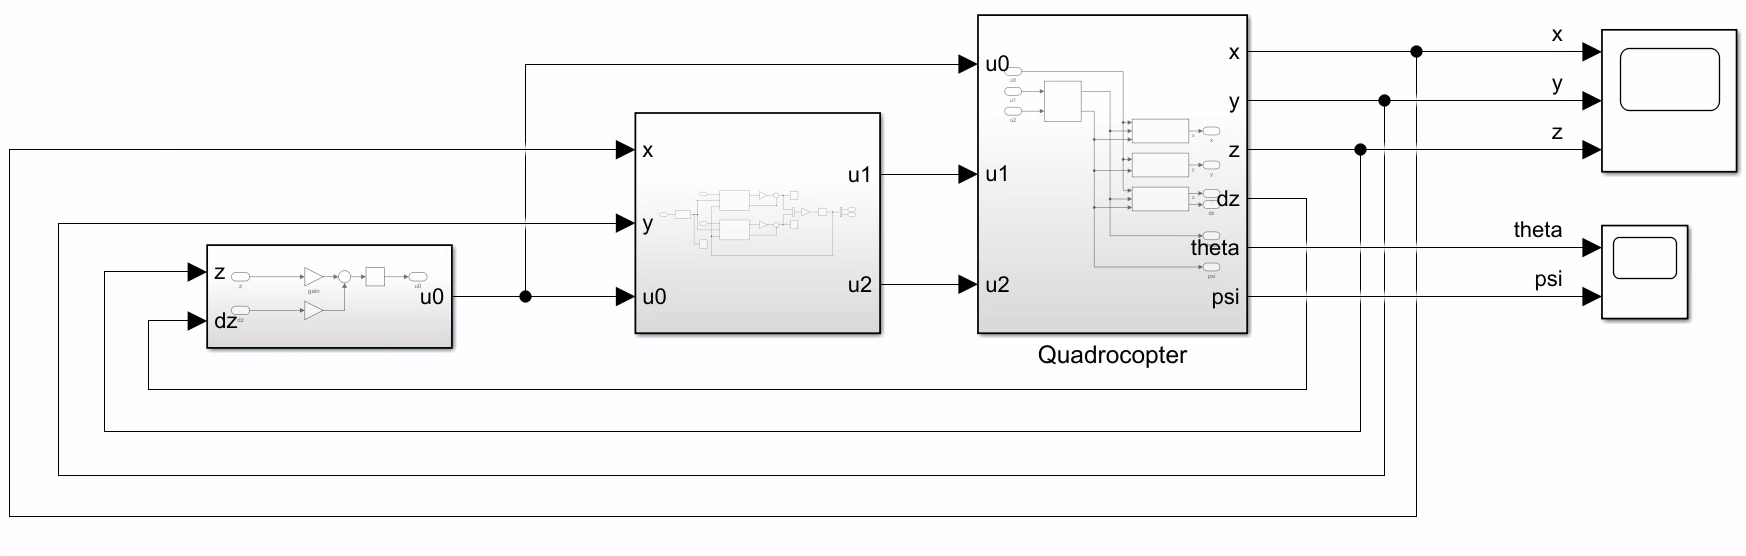
\includegraphics[width=\textwidth]{system.png}
        \caption{Модель управления квадрокоптером}
        \label{pic:system}
    \end{figure}

    \begin{figure}[H]
        \centering
        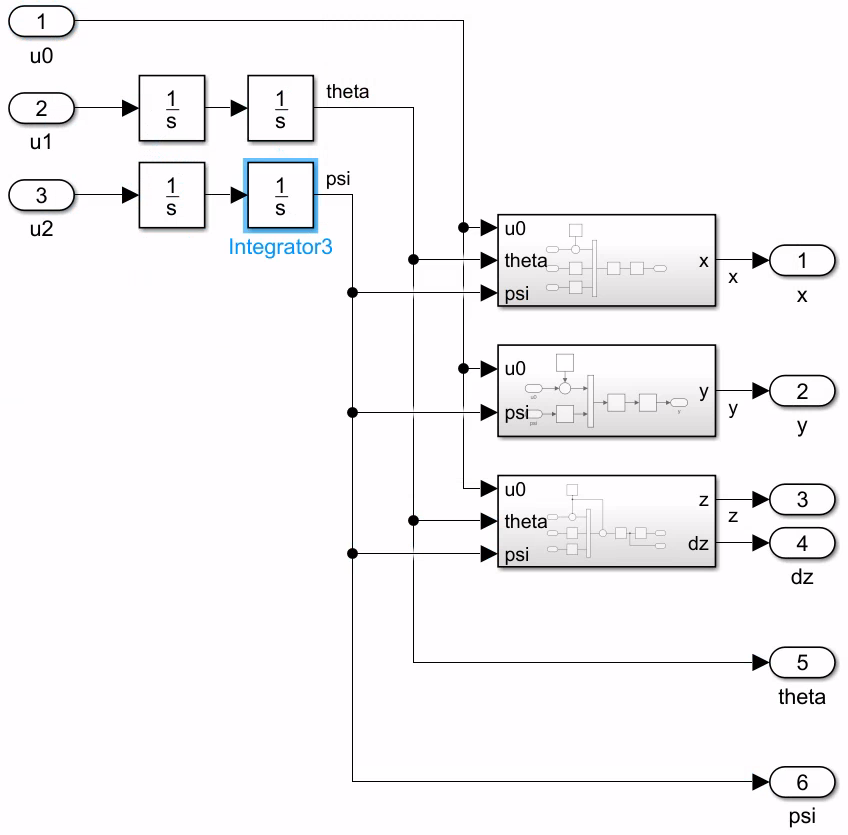
\includegraphics[width=0.75\textwidth]{quadro.png}
        \caption{Блок модели квадрокоптера}
        \label{pic:quadro}
    \end{figure}

    На рисунках~\ref{pic:x}-\ref{pic:z} представлены блоки определения координат квадрокоптера согласно~\eqref{eq:model}.
    \begin{figure}[H]
        \centering
        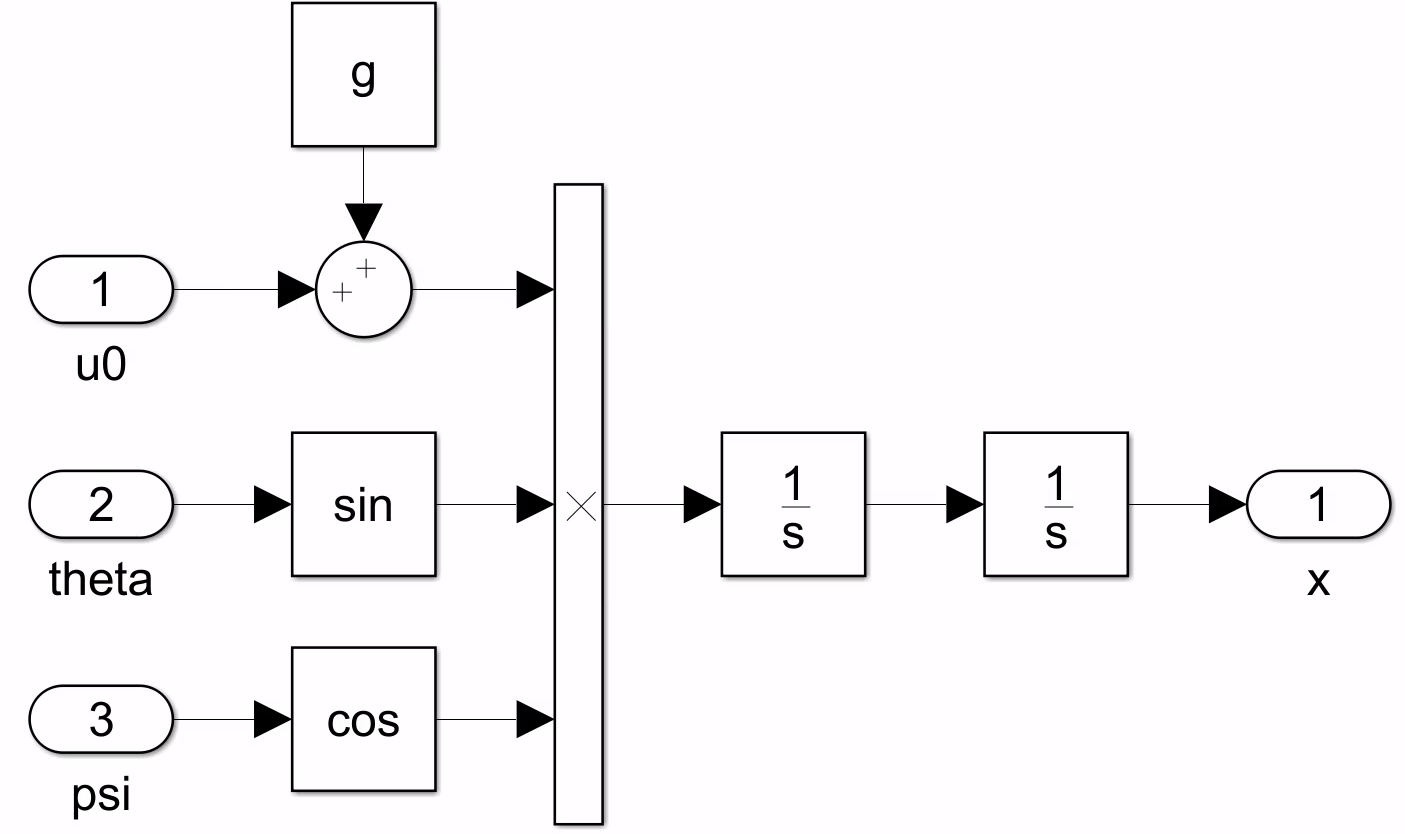
\includegraphics[height=0.2\textheight]{x.png}
        \caption{Блок определения координаты $x$}
        \label{pic:x}
    \end{figure}

    \begin{figure}[H]
        \centering
        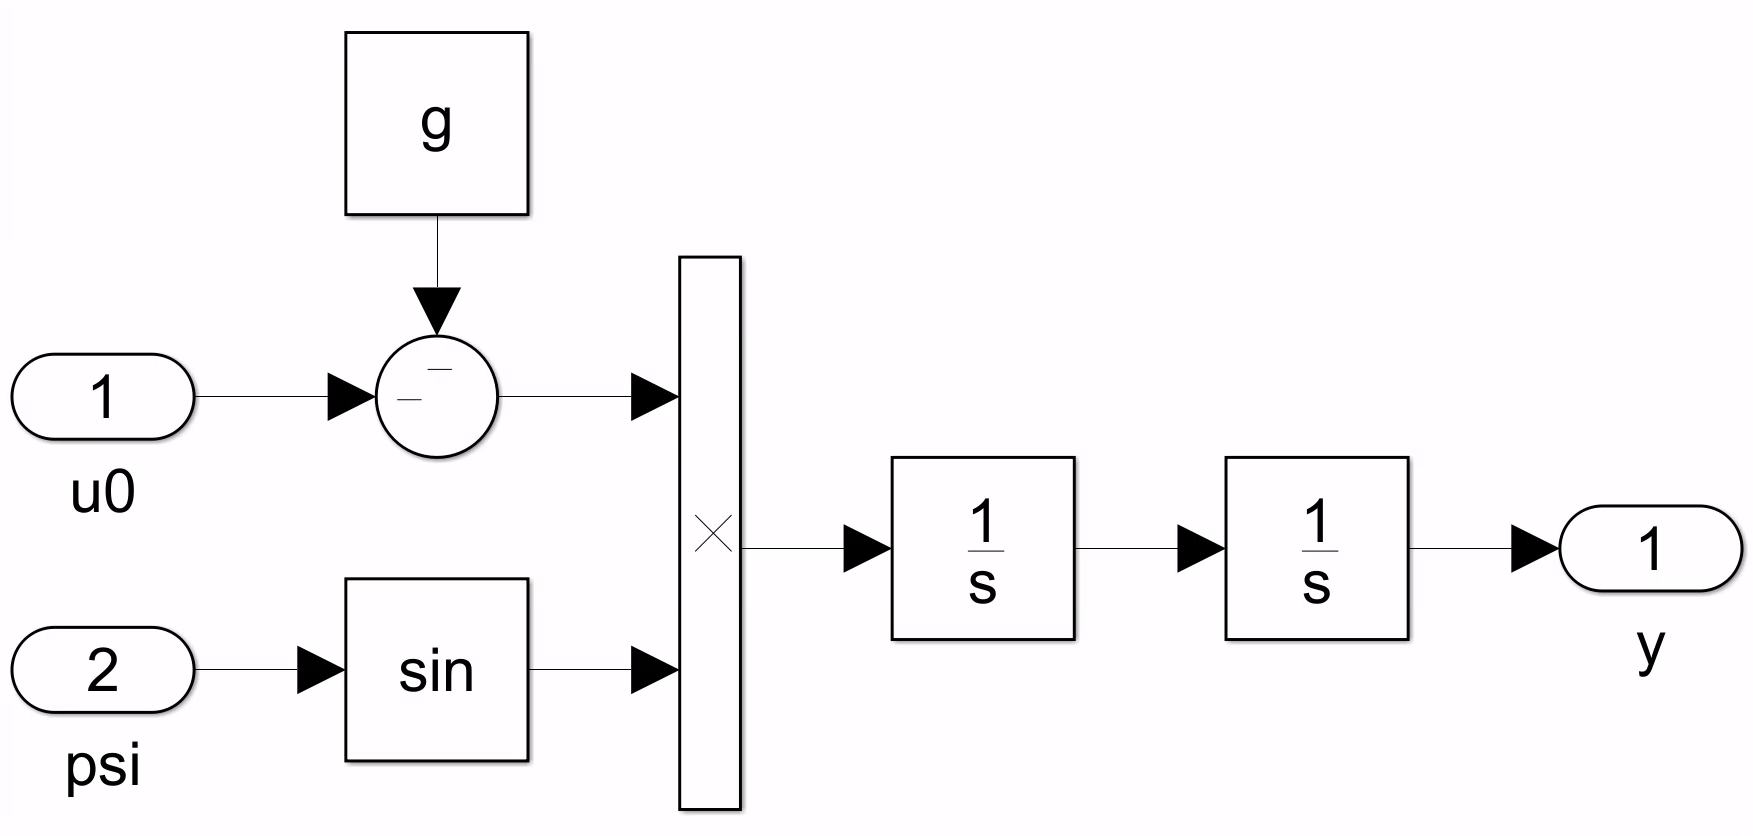
\includegraphics[height=0.2\textheight]{y.png}
        \caption{Блок определения координаты $y$}
        \label{pic:y}
    \end{figure}

    \begin{figure}[H]
        \centering
        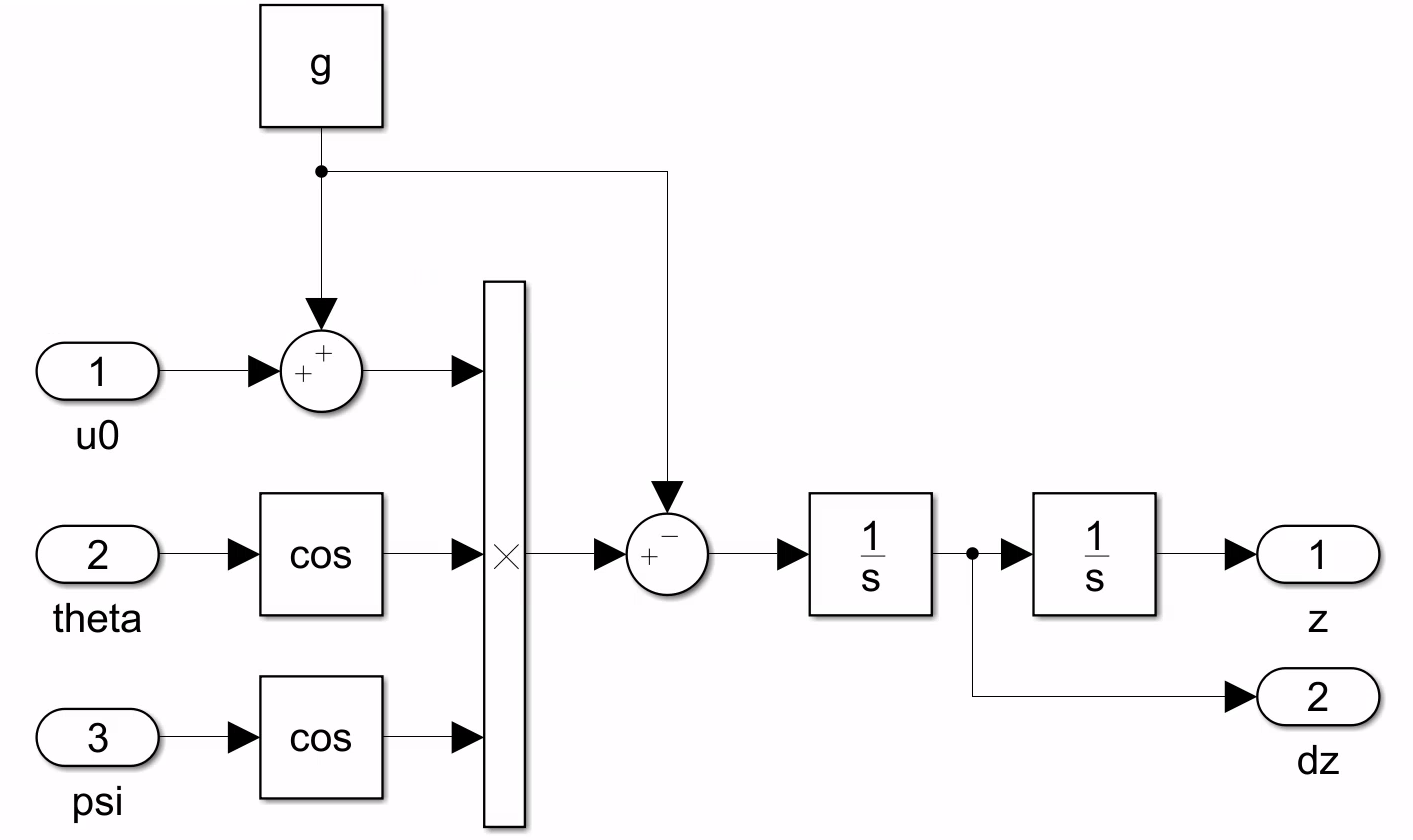
\includegraphics[height=0.3\textheight]{z.png}
        \caption{Блок определения координаты $z$}
        \label{pic:z}
    \end{figure}

    Регулятор по высоте выполненый по уравнению~\eqref{eq:u0}
    \begin{figure}[H]
        \centering
        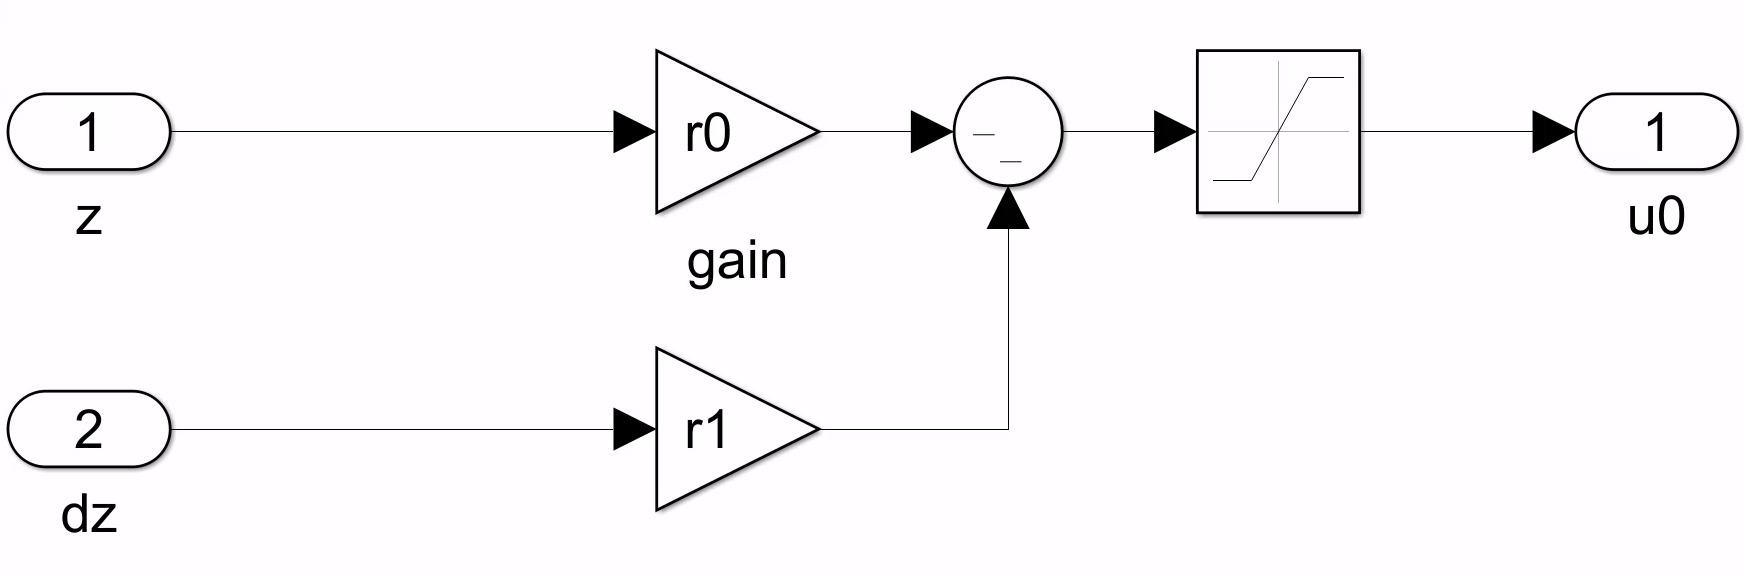
\includegraphics[width=\textwidth]{stabilizer.png}
        \caption{Блок регулятора по высоте}
        \label{pic:stab}
    \end{figure}

    Регулятор выполненый по системе~\eqref{eq:est u}
    \begin{figure}[H]
        \centering
        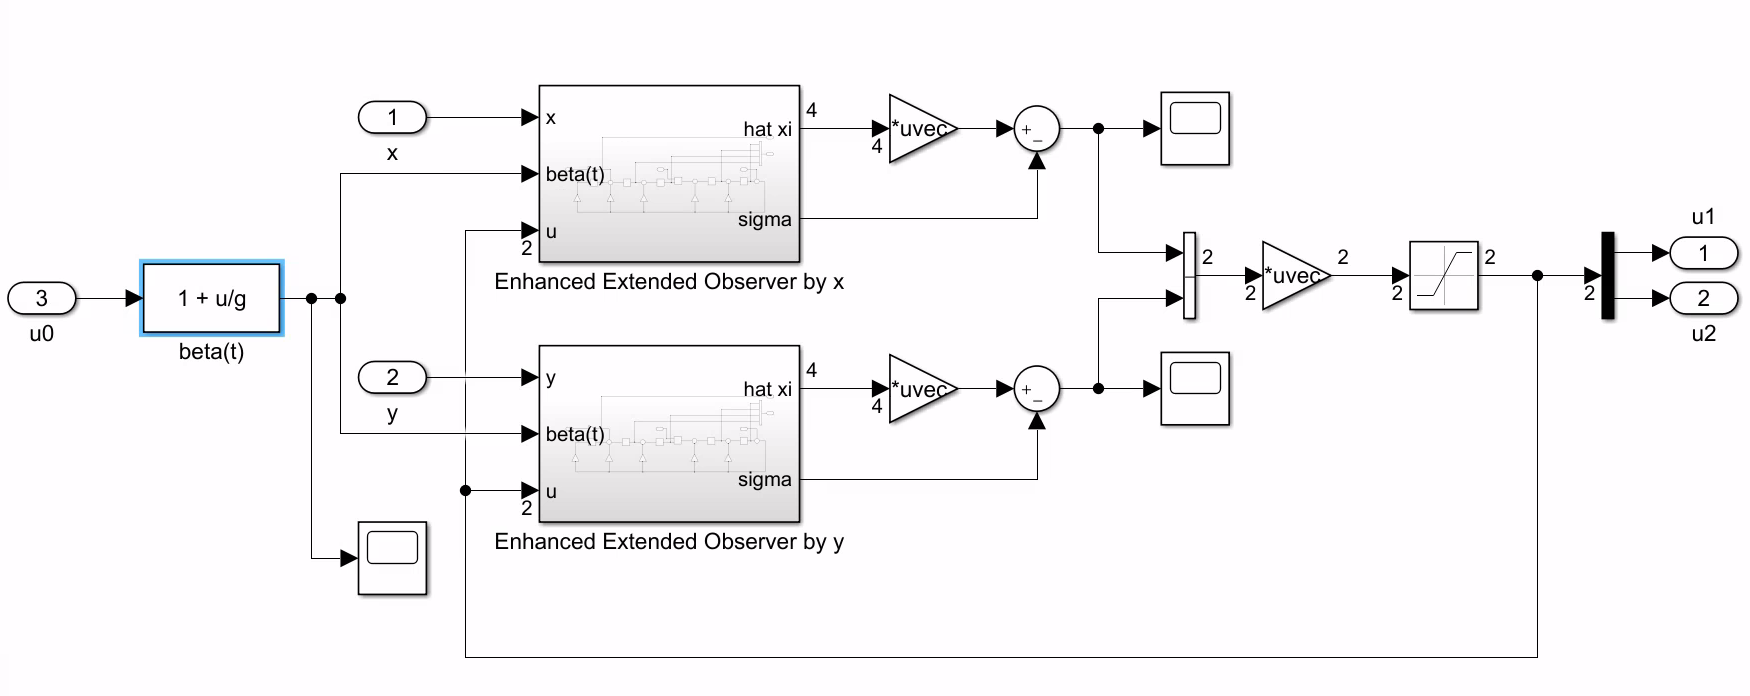
\includegraphics[width=0.75\textwidth]{u.png}
        \caption{Блок регулятора с УРН}
        \label{pic:u}
    \end{figure}

    Поскольку углы крена и тангажа неизмеримы, необходимо использовать УРН для каждого. Общее строение обоих блоков
    одинаково, поэтому приведём один (рисунок~\ref{pic:observer}). Данный блок позволяет найти оценку ускорения каждого
    угла, которую в свою очередь можно использовать для определения самого угла.

    \begin{figure}[H]
        \centering
        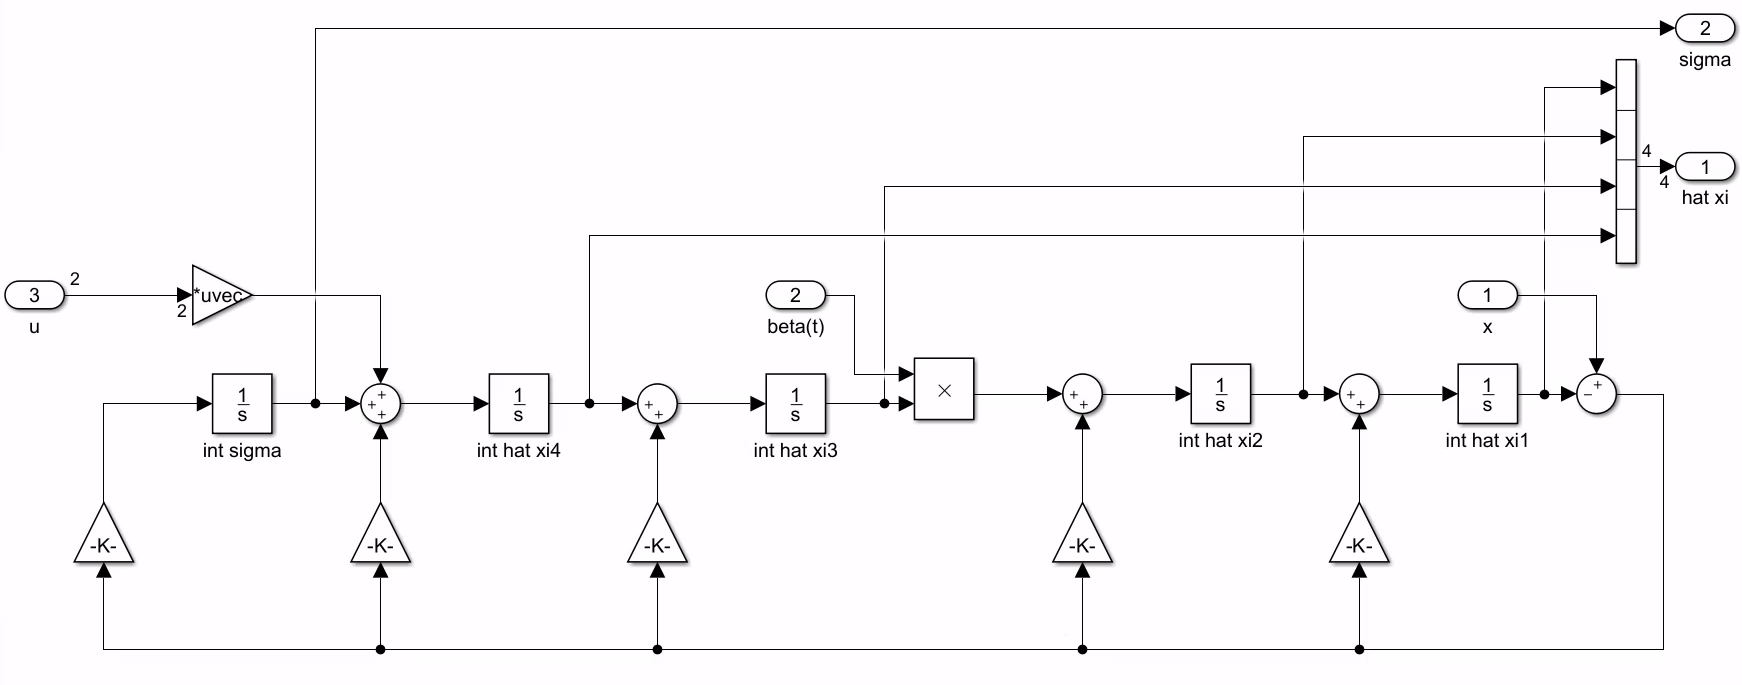
\includegraphics[width=0.75\textwidth]{observer.png}
        \caption{Блок УРН}
        \label{pic:observer}
    \end{figure}

    \section*{Результаты моделирования}

    \begin{figure}[H]
        \centering
        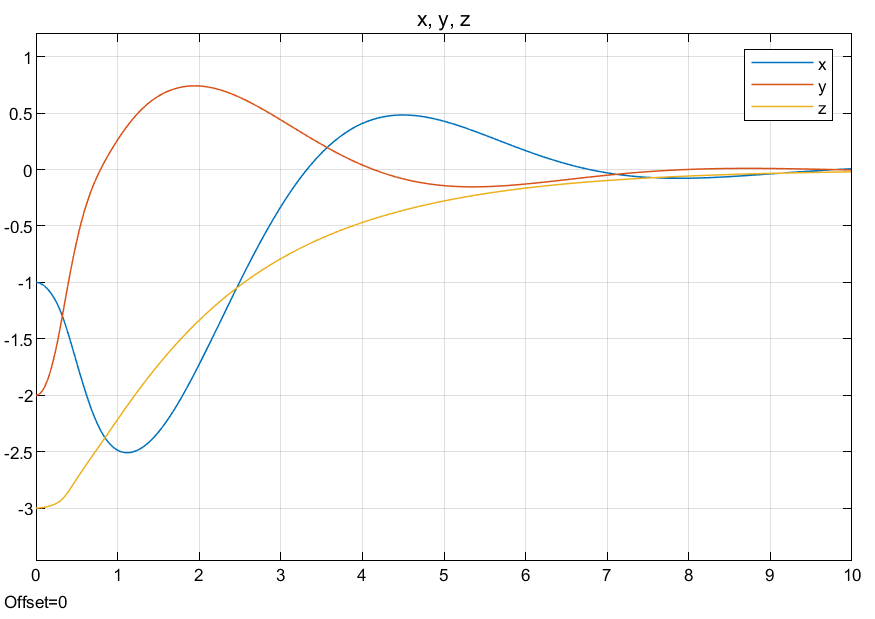
\includegraphics[width=0.75\textwidth]{xyz.png}
        \caption{Координаты квадрокоптера}
        \label{pic:xyz}
    \end{figure}

    \begin{figure}[H]
        \centering
        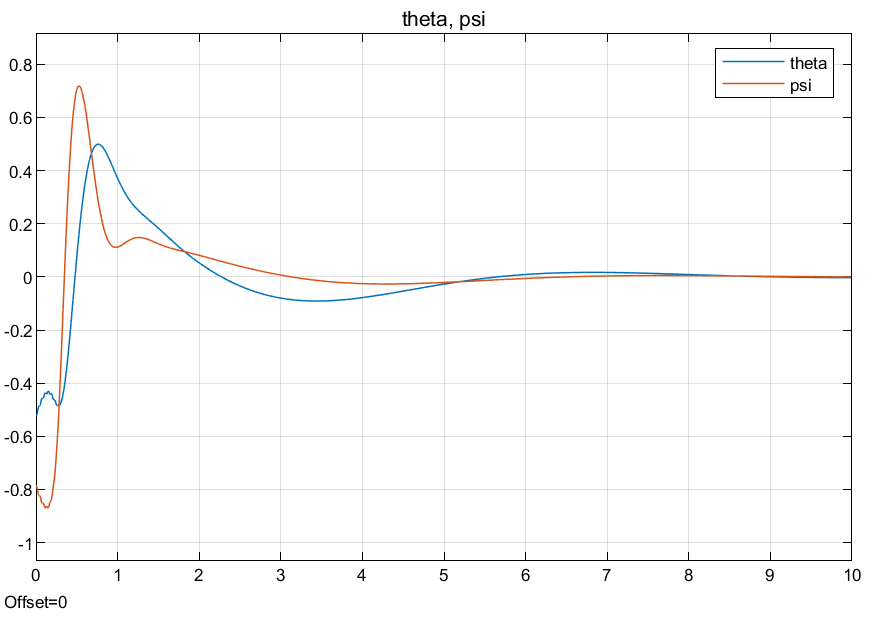
\includegraphics[width=0.75\textwidth]{angles.png}
        \caption{Углы квадрокоптера}
        \label{pic:angles}
    \end{figure}

    \begin{figure}[H]
        \centering
        \begin{subfigure}{0.49\textwidth}
            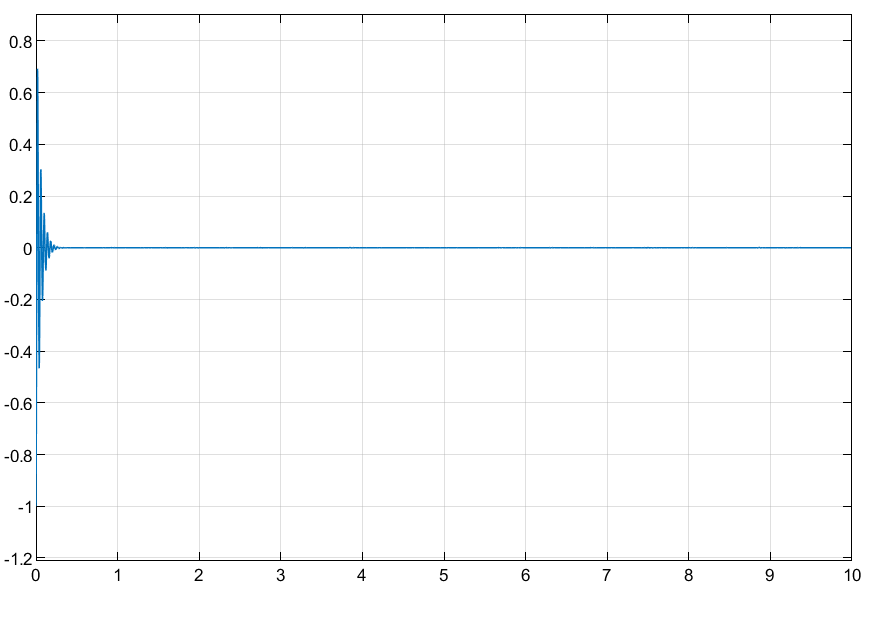
\includegraphics[width=\linewidth]{x eps.png}
            \caption{Ошибка по $x$}
        \end{subfigure}
        \begin{subfigure}{0.49\textwidth}
            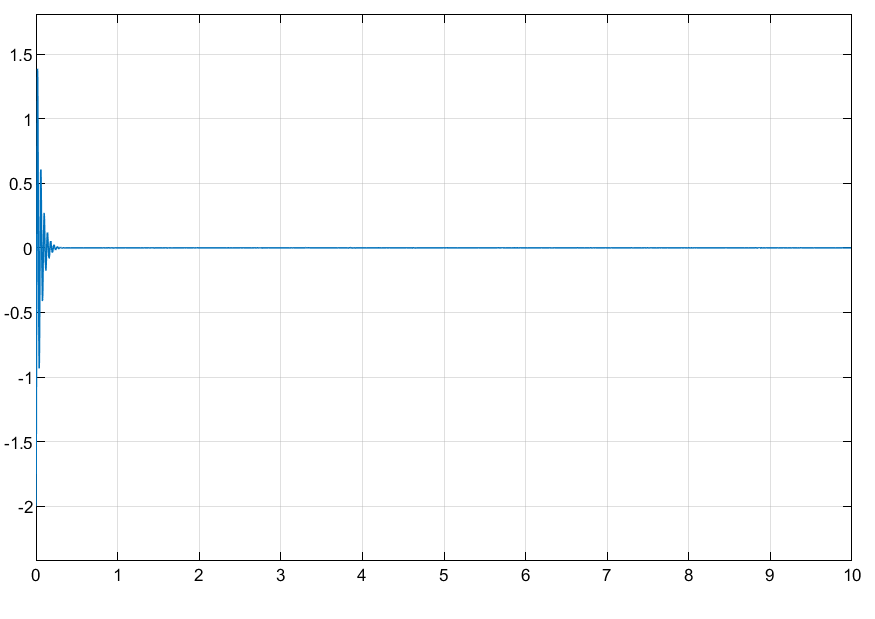
\includegraphics[width=\linewidth]{y eps.png}
            \caption{Ошибка по $y$}
        \end{subfigure}
        \caption{Ошибки регулирования}
        \label{pic:eps}
    \end{figure}

    \begin{figure}[H]
        \centering
        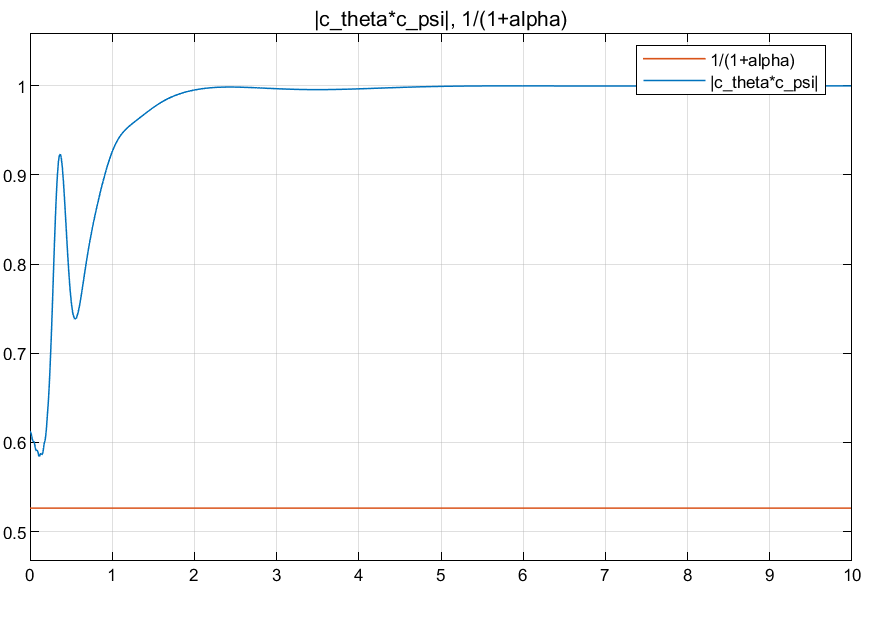
\includegraphics[width=0.75\textwidth]{abs(cc).png}
        \caption{Сравнение $\left| \cos\theta\cos\psi \right|$ и $\dfrac{1}{1+\alpha}$}
        \label{pic:abs(cc)}
    \end{figure}


    \section*{Вывод}
    В работе реализована модель удержания положения квадрокоптера на базе усовершенствованного расширенного наблюдателя.
    Результаты моделирования показывают, что координаты, углы и ошибки сходятся к нулю, что и было целью управления.
    Также по графикам видно, что выполняются поставленные ограничения $\left| \cos\theta\cos\psi \right| \ge \dfrac{1}{1+\alpha}$,
    $\left| \theta \right| < \dfrac{\pi}{2}$ и $\left| \psi \right| < \dfrac{\pi}{2}$.

    \appendix
    \renewcommand{\thesection}{\Asbuk{section}}
    \section{Скрипт инициализации модели}\label{code:given}
    \octavefile[frame=single]{../src/given.m}

\end{document}
